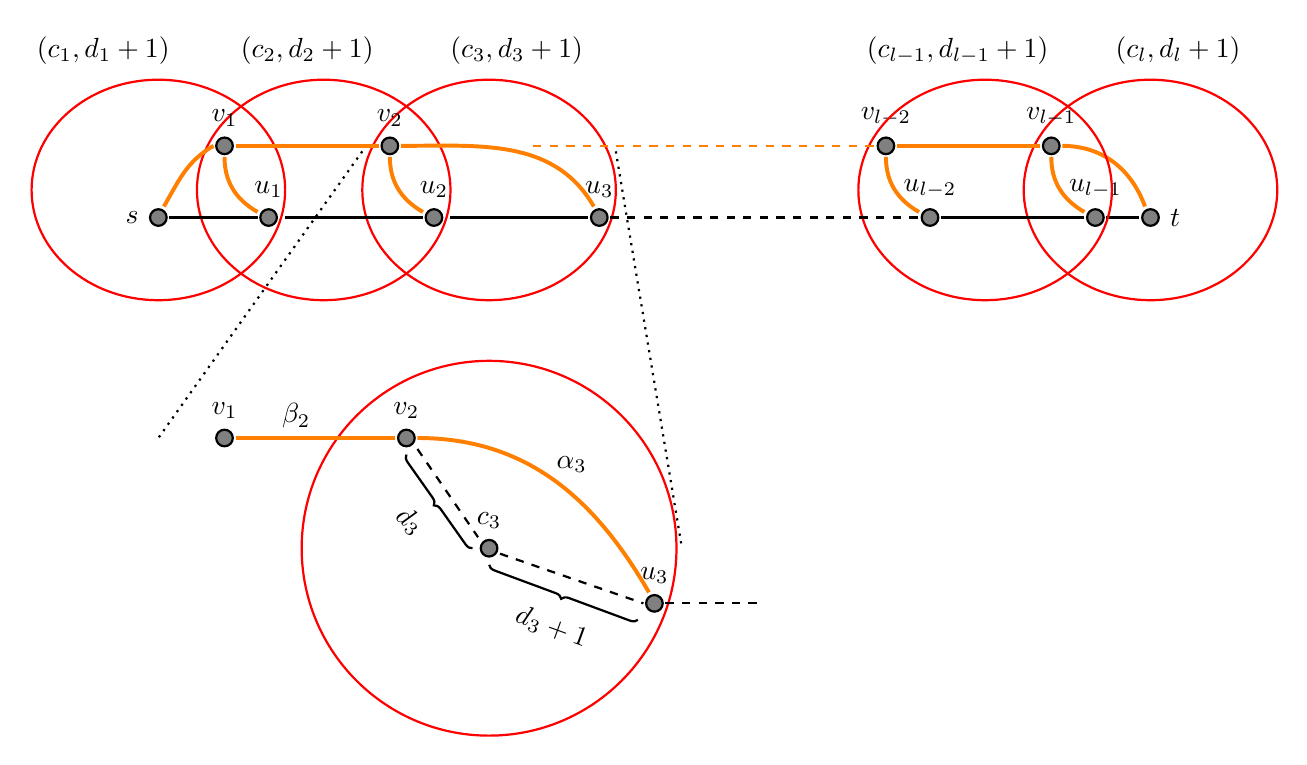
\begin{tikzpicture}[thick,scale=0.7]
	\draw [red] (0, 0.5) ellipse (2.3 and 2);
	\draw [red] (3, 0.5) ellipse (2.3 and 2);
	\draw [red] (6, 0.5) ellipse (2.3 and 2);
	\draw [red] (18, 0.5) ellipse (2.3 and 2);
	
	\draw (0, 0) node[circle, draw, fill=black!50, inner sep=0pt, minimum width=6pt, label = 180 : $s$] {};
	\draw (18, 0) node[circle, draw, fill=black!50, inner sep=0pt, minimum width=6pt,label = 0 : $t$] {};
	
	\draw (2, 0) node[circle, draw, fill=black!50, inner sep=0pt, minimum width=6pt,label = $u_1$] {};
	\draw (1.2, 1.3) node[circle, draw, fill=black!50, inner sep=0pt, minimum width=6pt,label = $v_1$] {};
	\draw [line width = 0.5mm] (0.2, 0) -- (1.8, 0);
	\draw [line width = 0.5mm, color=orange] (0.1, 0.2) to[out=60, in=210] (1, 1.3);
	\draw [line width = 0.5mm, color=orange] (1.2, 1.1) to[out=-90, in=150] (1.8, 0.1);
	
	\draw (-1, 2.4) node[red, label={$\ball(c_1, d_{1}+1)$}]{};
	
	\draw (5, 0) node[circle, draw, fill=black!50, inner sep=0pt, minimum width=6pt,label = $u_2$] {};
	\draw [line width = 0.5mm] (2.3, 0) -- (4.8, 0);
	
	\draw (2.7, 2.4) node[red, label={$\ball(c_2, d_{2}+1)$}]{};
	\draw [line width = 0.5mm, color=orange] (1.4, 1.3) -- (4, 1.3);
	\draw [line width = 0.5mm, color=orange] (4.2, 1.1) to[out=-90, in=150] (4.8, 0.1);
	
	\draw (4.2, 1.3) node[circle, draw, fill=black!50, inner sep=0pt, minimum width=6pt,label = $v_2$] {};
	\draw (8, 0) node[circle, draw, fill=black!50, inner sep=0pt, minimum width=6pt,label = $u_3$] {};
	\draw [line width = 0.5mm] (5.3, 0) -- (7.8, 0);
	
	\draw (6.5, 2.4) node[red, label={$\ball(c_3, d_{3}+1)$}]{};
	\draw [line width = 0.5mm, color=orange] (4.4, 1.3) to[out=0, in=120] (7.9, 0.2);
	
	\draw[dotted] (3.7, 1.2) -- (0, -4);
	\draw[dotted] (8.3, 1.2) -- (9.5, -6);
	\draw (4.5, -4) node[circle, draw, fill=black!50, inner sep=0pt, minimum width=6pt,label = $v_2$] {};
	\draw (9, -7) node[circle, draw, fill=black!50, inner sep=0pt, minimum width=6pt,label = $u_3$] {};
	\draw (6, -6) node[circle, draw, fill=black!50, inner sep=0pt, minimum width=6pt,label = $c_3$] {};
	\draw [red] (6, -6) ellipse (3.4 and 3.4);
	%\draw [dashed] (2, -7) -- (8.8, -7);	
	\draw [dashed] (9.2, -7) -- (11, -7);
	\draw [line width = 0.5mm, color=orange] (4.7, -4) to[out=0, in=120] (8.9, -6.8);
	\draw (7.5, -5) node[red, label={$\alpha_3$}]{};
	\draw [line width = 0.5mm, color=orange] (1.4, -4) to (4.3, -4);
	\draw (1.2, -4) node[circle, draw, fill=black!50, inner sep=0pt, minimum width=6pt,label = $v_1$] {};
	\draw (2.5, -4.2) node[red, label={$\beta_2$}]{};
	
	\draw [decorate, decoration = {brace}] (5.7,-6) -- (4.5,-4.3);
	\draw [dashed] (4.7, -4.2) -- (5.8, -5.8);
	\draw (4.3, -6) node[label={[rotate=-40]$d_3$}]{};
	\draw [decorate, decoration = {brace}] (8.7, -7.3) -- (6, -6.3);
	\draw [dashed] (6.2, -6.1) -- (8.8, -7);
	\draw (7, -8) node[label={[rotate=-20]$d_3+1$}]{};
	
	\draw (16.2, 1.3) node[circle, draw, fill=black!50, inner sep=0pt, minimum width=6pt,label = $v_{l-1}$] {};
	\draw (17, 0) node[circle, draw, fill=black!50, inner sep=0pt, minimum width=6pt,label = $u_{l-1}$] {};
	\draw [line width = 0.5mm] (17.8, 0) -- (17.2, 0);
	
	\draw [line width = 0.5mm, color=orange] (16.4, 1.3) to[out=0, in=110] (17.9, 0.2);
	
	\draw (18.5, 2.4) node[red, label={$\ball(c_l, d_{l}+1)$}]{};
	
	\draw (13.2, 1.3) node[circle, draw, fill=black!50, inner sep=0pt, minimum width=6pt,label = $v_{l-2}$] {};
	\draw (14, 0) node[circle, draw, fill=black!50, inner sep=0pt, minimum width=6pt,label = $u_{l-2}$] {};
	\draw [line width = 0.5mm] (16.8, 0) -- (14.2, 0);
	\draw [red] (15, 0.5) ellipse (2.3 and 2);
	\draw (14.5, 2.4) node[red, label={$\ball(c_{l-1}, d_{l-1}+1)$}]{};
	\draw [line width = 0.5mm, color=orange] (13.2, 1.1) to[out=-90, in=150] (13.8, 0.1);
	\draw [line width = 0.5mm, color=orange] (13.4, 1.3) -- (16, 1.3);
	\draw [line width = 0.5mm, color=orange] (16.2, 1.1) to[out=-90, in=150] (16.8, 0.1);
	
	\draw [dashed, color=orange] (6.8, 1.3) -- (13.1, 1.3);
	\draw [dashed] (8.2, 0) -- (13.8, 0);
\end{tikzpicture}